\documentclass[tikz,border=2pt]{standalone}
\usepackage{amsmath,amssymb}
\usepackage{tikz}
\usepackage{pgfplots}
\pgfplotsset{compat=1.18}

\begin{document}
% Uniform demand on [80,120]: constant density 1/40; the probability beta = 0.6 is the shaded
% rectangle from 80 to y* = 80 + 40 x 0.6 = 104.
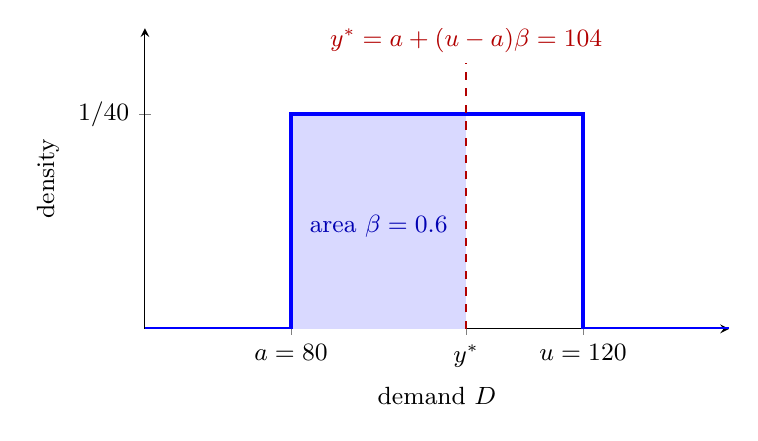
\begin{tikzpicture}
	\begin{axis}[width=9cm, height=5.4cm, xlabel={demand $D$}, ylabel={density}, xmin=60, xmax=140, ymin=0, ymax=0.035, axis lines=left, tick label style={font=\small}, label style={font=\small}, xtick={80,104,120}, xticklabels={$a=80$,$y^*$,$u=120$}, ytick={0.025}, yticklabels={$1/40$}, scaled y ticks=false]
		\fill[blue!15] (axis cs:80,0) rectangle (axis cs:104,0.025);
		\addplot[blue, very thick] coordinates {(60,0) (80,0) (80,0.025) (120,0.025) (120,0) (140,0)};
		\draw[red!70!black, dashed, thick] (axis cs:104,0) -- (axis cs:104,0.031);
		\node[font=\small, blue!70!black] at (axis cs:92,0.012) {area $\beta=0.6$};
		\node[anchor=south, font=\small, red!70!black] at (axis cs:104,0.031) {$y^*=a+(u-a)\beta=104$};
	\end{axis}
	\end{tikzpicture}
\end{document}
